\documentclass[tikz,border=0pt]{standalone}
% rppreamble.tex -- engine switch for the standalone figure builds.
% Tectonic/XeTeX loads xeCJK; pdfLaTeX (arXiv) loads CJKutf8 with gbsn.
% Every Chinese string goes through \zh{...}. main.tex repeats this switch,
% and the standalone package skips this preamble when main.tex inputs a figure.
\usepackage{iftex}
\ifXeTeX
  \usepackage{xeCJK}
  \setCJKmainfont{FandolSong-Regular.otf}
  \setCJKsansfont{FandolHei-Regular.otf}
  \setCJKmonofont{FandolHei-Regular.otf}
  \providecommand{\zh}[1]{#1}
\else
  \usepackage[T1]{fontenc}
  \usepackage[utf8]{inputenc}
  \usepackage{lmodern}
  \usepackage{CJKutf8}
  \DeclareRobustCommand{\zh}[1]{\begin{CJK}{UTF8}{gbsn}#1\end{CJK}}
\fi
\usepackage{amsmath,amssymb}
\usepackage{xcolor}
\usepackage{tikz}
% rpstyle.tex -- the one visual system shared by every ReadProof figure.
% Loaded by each standalone figure (through rppreamble.tex) and by main.tex.
% Palette: ink #03080a for text and plain flow; violet #5b4be8 for ReadProof
% components; red #e2452a for walls and failures; greys for neutral parts.
% Labels are set at 8--8.5 pt so they stay readable at 100% in the paper.
\usetikzlibrary{positioning,arrows.meta,calc,shapes.geometric,shapes.misc,fit,backgrounds}
\definecolor{rpInk}{HTML}{03080A}
\definecolor{rpViolet}{HTML}{5B4BE8}
\definecolor{rpRed}{HTML}{E2452A}
\definecolor{rpGrey}{HTML}{8C929B}
\definecolor{rpGreyDark}{HTML}{50565E}
\definecolor{rpGreyFill}{HTML}{F2F3F5}
\definecolor{rpVioletFill}{HTML}{ECE9FC}
\definecolor{rpVioletPale}{HTML}{F8F7FE}
\definecolor{rpRedFill}{HTML}{FCE9E5}
\providecommand{\rpfont}{\fontsize{8.5}{10}\selectfont\sffamily}
\providecommand{\rpsmall}{\fontsize{8}{9.4}\selectfont\sffamily}
\providecommand{\rpmono}{\fontsize{7.8}{9.2}\selectfont\ttfamily}
\providecommand{\rpdot}{\,\ensuremath{\cdot}\,}
\providecommand{\rpto}{\ensuremath{\rightarrow}}
\providecommand{\rpt}[1]{{\fontsize{8.5}{10.2}\selectfont\bfseries #1}}% node title
\tikzset{
  rp base/.style={rounded corners=3pt, line width=0.6pt, align=center,
    inner xsep=4pt, inner ysep=2.6pt, font=\rpsmall, text=rpInk,
    execute at begin node={\hyphenpenalty=10000\exhyphenpenalty=10000}},
  neutral/.style={rp base, draw=rpGrey, fill=rpGreyFill},
  rp/.style={rp base, draw=rpViolet, fill=rpVioletFill},
  rp strong/.style={rp base, draw=rpViolet, fill=rpViolet, text=white},
  rp gate/.style={rp base, draw=rpViolet, fill=rpVioletFill, line width=1.15pt},
  wall/.style={rp base, draw=rpRed, fill=rpRedFill},
  wall strong/.style={rp base, draw=rpRed, fill=rpRed, text=white},
  data/.style={rp base, draw=rpGrey, fill=white, font=\rpmono, align=left},
  store/.style={cylinder, shape border rotate=90, aspect=0.07, draw=rpViolet,
    fill=rpVioletFill, line width=0.6pt, align=center, font=\rpsmall,
    text=rpInk, inner xsep=4pt, inner ysep=1pt,
    execute at begin node={\hyphenpenalty=10000\exhyphenpenalty=10000}},
  flow/.style={-{Stealth[length=5pt,width=4pt]}, line width=0.7pt, draw=rpInk},
  rpflow/.style={flow, draw=rpViolet},
  wallflow/.style={flow, draw=rpRed},
  logflow/.style={-{Stealth[length=4pt,width=3.5pt]}, line width=0.55pt,
    draw=rpGrey, dash pattern=on 2.6pt off 1.8pt},
  assoc/.style={line width=0.7pt, draw=rpViolet},
  edge label/.style={font=\rpsmall, text=rpGreyDark, inner sep=1.2pt},% no fill: place clear of lines
  wall label/.style={edge label, text=rpRed, fill=white},% white patch: may sit across a panel border
  group/.style={rounded corners=6pt, draw=rpViolet!35, fill=rpVioletPale,
    line width=0.5pt},
  group label/.style={font=\rpsmall\bfseries, text=rpViolet},
  panel title/.style={font=\fontsize{9}{11}\selectfont\sffamily\bfseries, text=rpInk},
}

% Opaque white page under everything, for the standalone PDFs and PNG checks
% only (main.tex never reads this preamble). A layer below "background" keeps
% the pale group panels visible.
\pgfdeclarelayer{rppage}
\pgfsetlayers{rppage,background,main}
\tikzset{every picture/.append style={execute at end picture={%
  \begin{pgfonlayer}{rppage}\fill[white]
    ([shift={(-2pt,-2pt)}]current bounding box.south west) rectangle
    ([shift={(2pt,2pt)}]current bounding box.north east);\end{pgfonlayer}}}}

\begin{document}
% The ReadProof v1 evaluation pipeline (2026-11-21). Top row: the three inputs, combined by a
% product, fill the run matrix, which runs live once and is replayed for scoring. One return
% line carries both arms' runs to the bottom row: logs, scorer, metrics,
% leaderboard. Both rows read left to right.
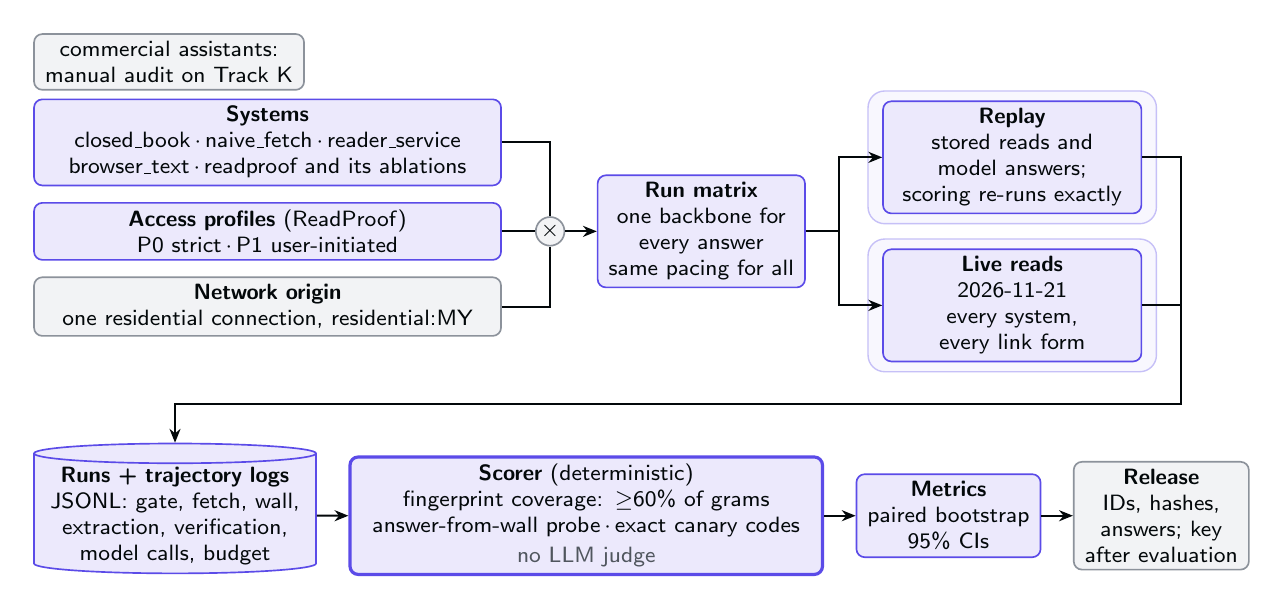
\begin{tikzpicture}[node distance=0.4cm,
  op/.style={neutral, circle, inner sep=0.6pt, font=\rpfont},
  merge/.style={flow, -},
  lane/.style={group, inner xsep=0.18cm, inner ysep=0.12cm},
]
\def\iw{5.65cm}% input text width
\def\aw{3.0cm}% arm text width
% ---------------- inputs (stacked) ----------------
\node[rp, text width=\iw] (SY) at (0,0)
  {\rpt{Systems}\\closed\_book\rpdot naive\_fetch\rpdot reader\_service\\
   browser\_text\rpdot readproof and its ablations};
% Commercial assistants sit beside the systems but outside the run matrix
% (audited by hand), so their note has no edge into the product.
\node[neutral, anchor=south west] (CA) at ($(SY.north west)+(0,0.1)$)
  {commercial assistants:\\manual audit on Track K};
\node[rp, text width=\iw, below=0.2cm of SY] (AP)
  {\rpt{Access profiles} (ReadProof)\\P0 strict\rpdot P1 user-initiated};
\node[neutral, text width=\iw, below=0.2cm of AP] (NO)
  {\rpt{Network origin}\\one residential connection, residential:MY};
\node[op, right=0.42cm of AP] (X) {$\times$};
% ---------------- run matrix and the two arms ----------------
\node[rp, right=0.4cm of X] (RM)
  {\rpt{Run matrix}\\one backbone for\\every answer\\same pacing for all};
\node[rp, text width=\aw, anchor=west] (FR) at ($(RM.east)+(0.97,0.94)$)
  {\rpt{Replay}\\stored reads and\\model answers;\\scoring re-runs exactly};
\node[rp, text width=\aw, anchor=west] (LV) at ($(RM.east)+(0.97,-0.94)$)
  {\rpt{Live reads}\\2026-11-21\\every system,\\every link form};
\begin{scope}[on background layer]
  \node[lane, fit=(FR)] (gFR) {};
  \node[lane, fit=(LV)] (gLV) {};
\end{scope}
% ---------------- bottom row ----------------
\coordinate (ch) at ($(gLV.south)+(0,-0.4)$);% the return line runs here
\node[store, text width=3.3cm, anchor=west] (LOG) at ($(SY.west |- ch)+(0,-1.42)$)
  {\rpt{Runs + trajectory logs}\\JSONL:\ gate, fetch, wall,\\extraction, verification,\\model calls, budget};
\node[rp gate, text width=5.72cm, right=of LOG] (SC)
  {\rpt{Scorer} (deterministic)\\fingerprint coverage: $\ge$60\% of grams\\
   answer-from-wall probe\rpdot exact canary codes\\[1.5pt]
   {\color{rpGreyDark}no LLM judge}};
\node[rp, right=of SC] (MT) {\rpt{Metrics}\\paired bootstrap\\95\% CIs};
\node[neutral, right=of MT] (LB) {\rpt{Release}\\IDs, hashes,\\answers; key\\after evaluation};
% ---------------- flows ----------------
\draw[merge] (SY.east) -| (X.north);
\draw[merge] (NO.east) -| (X.south);
\draw[merge] (AP.east) -- (X.west);
\draw[flow] (X.east) -- (RM.west);
\draw[flow] (RM.east) -- ++(0.42,0) |- (FR.west);
\draw[flow] (RM.east) -- ++(0.42,0) |- (LV.west);
\coordinate (jx) at ($(gFR.east)+(0.3,0)$);
\draw[merge] (LV.east) -- (LV.east -| jx);
\draw[flow] (FR.east) -- (FR.east -| jx) -- (jx |- ch) -- (LOG.north |- ch) -- (LOG.north);
\draw[flow] (LOG) -- (SC);
\draw[flow] (SC) -- (MT);
\draw[flow] (MT) -- (LB);
\end{tikzpicture}
\end{document}
